\chapter{Transformada de Laplace}
\section{Definição de transformada de Laplace}{\label{sec_1}}
\begin{defn}Seja $f(t)$ uma função definida nos reais não negativos. Quando a integral
$$
{\mathcal{L}}\{f(t)\}=\int_0^\infty f(t)e^{-st}dt
$$
for convergente, ela será chamada de transformada de Laplace da função $f(t)$.
\end{defn}
A transformada de Laplace $\mathcal{L}\{f(t)\}$ de uma função $f(t)$ é uma função da variável $s$. A notação usual neste contexto é letra minúscula para a função e letra maiúscula para a transformada: $\mathcal{L}\{f(t)\}=F(s)$, $\mathcal{L}\{g(t)\}=G(s)$, $\mathcal{L}\{h(t)\}=H(s)$.
Nos próximos exemplos, vamos aplicar a definição para calcular a transformadas de Laplace de algumas funções.
\begin{ex}\label{ex1} Vamos calcular a transformada de Laplace da função $f(t)=1$:
\begin{eqnarray*}
\mathcal{L}\{1\}&=&\int_0^\infty 1\cdot e^{-st}dt\\
&=&\lim_{a\to\infty}\int_0^a  e^{-st}dt\\
&=&\lim_{a\to\infty} \frac{1-e^{-sa}}{s}.\\
\end{eqnarray*}
O limite $\displaystyle\lim_{a\to\infty}\frac{1-e^{-sa}}{s}$ só existe se $s>0$. Portanto,
\begin{eqnarray*}
\mathcal{L}\{1\}=\frac{1}{s},\qquad s>0.\\
\end{eqnarray*}
\end{ex}
\begin{ex}\label{ex2} A transformada de Laplace da função $f(t)=t$ é calculada fazendo integração por partes:
\begin{eqnarray*}
\mathcal{L}\{t\}&=&\int_0^\infty te^{-st}dt\\
&=&\left.-\frac{te^{-st}}{s}\right|_0^\infty-\int_0^\infty \left(-\frac{e^{-st}}{s}\right)dt .\\
&=&\left.-\frac{te^{-st}}{s}\right|_0^\infty+\frac{1}{s}\int_0^\infty e^{-st}dt .\\
\end{eqnarray*}
onde a notação $\displaystyle\left.-\frac{te^{-st}}{s}\right|_0^\infty$ indica $\displaystyle\lim_{a\to\infty}\left(\left.-\frac{te^{-st}}{s} \right|_0^a\right)$. Observe que, se $s>0$, a primeira parcela do lado direito é zero e a segunda é $\frac{1}{s}\mathcal{L}\{1\}$, isto é,
\begin{eqnarray*}
\mathcal{L}\{t\}&=&\frac{1}{s}\mathcal{L}\{1\}=\frac{1}{s^2},\qquad s>0.\\
\end{eqnarray*}
onde usamos o resultado do exemplo \ref{ex1}.
\end{ex}
\begin{ex} Para calcular a transformada de Laplace da função $f(t)=t^n$ usamos a ideia introduzida no exemplo \ref{ex2} e escrevemos-a em termos da transformada de $t^{n-1}$. Observe primeiro a transformada de $t^2$ e $t^3$
\begin{eqnarray*}
\mathcal{L}\{t^2\}&=&\int_0^\infty t^2e^{-st}dt\\
&=&\left.-\frac{t^2 e^{-st}}{s}\right|_0^\infty-\int_0^\infty \left(-2t\frac{e^{-st}}{s}\right)dt .\\
&=&\frac{2}{s}\int_0^\infty te^{-st}dt=\frac{2}{s}\mathcal{L}\{t\}=\frac{2}{s}\frac{1}{s^2}=\frac{2}{s^3},\qquad s>0
\end{eqnarray*}
\begin{eqnarray*}
\mathcal{L}\{t^3\}&=&\int_0^\infty t^3e^{-st}dt\\
&=&\left.-\frac{t^3 e^{-st}}{s}\right|_0^\infty-\int_0^\infty \left(-3t^2\frac{e^{-st}}{s}\right)dt .\\
&=&\frac{3}{s}\int_0^\infty t^2e^{-st}dt=\frac{3}{s}\mathcal{L}\{t^2\}=\frac{3}{s}\frac{2}{s^3}=\frac{3!}{s^4},\qquad s>0
\end{eqnarray*}
Agora já podemos intuir qual seria a expressão para a transformada de $t^n$:
$$
\mathcal{L}\{t^n\}=\frac{n!}{s^{n+1}},\qquad s>0.
$$
Essa expressão pode ser formalmente demonstrada pelo método de indução matemática (ver exercício \ref{inducao_tn}).
\end{ex}
\begin{ex}{\label{ex_trans_exp}}A transformada de Laplace da função $f(t)=e^{-at}$ pode ser obtida por integração direta:
\begin{eqnarray*}
\mathcal{L}\{e^{-at}\}&=&\int_0^\infty e^{-at}e^{-st}dt\\
&=&\int_0^\infty e^{-(s+a)t}dt\\
&=&\left.\frac{e^{-(s+a)t}}{s+a}\right|_0^\infty=\frac{1}{s+a},\qquad s+a>0
\end{eqnarray*}
\end{ex}
\begin{ex}{\label{ex_trans_sin}}A transformada de Laplace da função $f(t)=\sen(w t)$ pode ser obtida integrando por partes duas vezes:
\begin{eqnarray*}
\mathcal{L}\{\sen(wt)\}&=&\int_0^\infty \sen(wt)e^{-st}dt\\
&=&\left.-\frac{\sen(wt)e^{-st}}{s}\right|_0^\infty-\frac{1}{s}\int_0^\infty \left(w\cos(wt)\right)\left(-e^{-st}\right)dt\\
&=&\frac{w}{s}\int_0^\infty \cos(wt)e^{-st}dt\\
&=&\frac{w}{s}\left(\left.-\frac{\cos(wt)e^{-st}}{s}\right|_0^\infty-\frac{1}{s}\int_0^\infty \left(-w\sen(wt)\right)\left(-e^{-st}\right)dt\right)\\
&=&\frac{w}{s}\left(\frac{1}{s}-\frac{w}{s}\int_0^\infty \sen(wt)e^{-st}dt\right)\\
&=&\frac{w}{s^2}-\frac{w^2}{s^2}\mathcal{L}\{\sen(wt)\} .
\end{eqnarray*}
Observe que obtemos uma equação para $\mathcal{L}\{\sen(wt)\}$:
$$
\mathcal{L}\{\sen(wt)\} =\frac{w}{s^2}-\frac{w^2}{s^2}\mathcal{L}\{\sen(wt)\} .
$$
Resolvemos essa equação e obtemos
$$
\mathcal{L}\{\sen(wt)\}\left(1+\frac{w^2}{s^2}\right)=\frac{w}{s^2},
$$
isto é,
$$
\mathcal{L}\{\sen(wt)\}=\frac{w}{s^2+w^2},\qquad s>0.
$$
\end{ex}
\begin{ex} Vamos agora calcular a transformada de Laplace $\mathcal{L}\{f(t)\}$ de uma função $f(t)$ descontínua definida por partes:
$$
f(t)=\left\{\begin{array}{ll} 0, &0\leq t\leq 4\\ 5, & t> 4.
\end{array}\right.
$$
Aqui usamos a seguinte propriedade de integral: $\int_a^b f(t)dt=\int_a^x f(t)dt+\int_x^b f(t)dt$. Portanto,
\begin{eqnarray*}
\mathcal{L}\{f(t)\}&=&\int_0^\infty f(t)e^{-st}dt\\
&=&\int_0^4 f(t)e^{-st}dt+\int_4^\infty f(t)e^{-st}dt\\
&=&\int_0^4 0\cdot e^{-st}dt+\int_4^\infty 5 e^{-st}dt\\
&=&\left.-\frac{5e^{-st}}{s}\right|_4^\infty=\frac{5e^{-4s}}{s}
\end{eqnarray*}
\end{ex}

\subsection*{Exercícios}
\begin{exer}Calcule a transforma de Laplace da função $f(t)=\cos(wt)$ usando a definição. 
\end{exer}
\begin{exer}Calcule a transforma de Laplace da função $f(t)$ definida por partes:
$$
f(t)=\left\{\begin{array}{ll} 0, &0\leq t\leq 3\\ 1, & 3\leq t\leq 5,\\0,&t>5.
\end{array}\right.
$$
\end{exer}
\begin{exer}{\label{ex_cap_3_1}} Use a definição de transformada de Laplace para calcular as transformadas das funções dadas nos gráficos abaixo:
\begin{center}

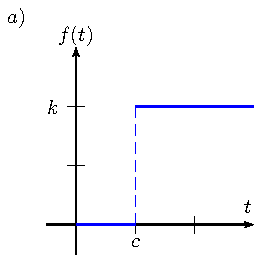
\includegraphics{cap_definicao/pics/figura_4}
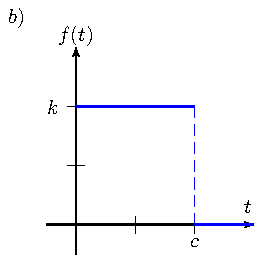
\includegraphics{cap_definicao/pics/figura_5}
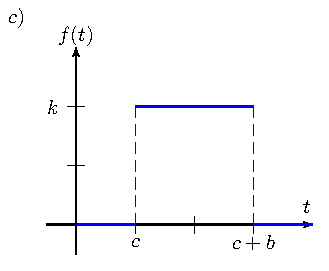
\includegraphics{cap_definicao/pics/figura_6}
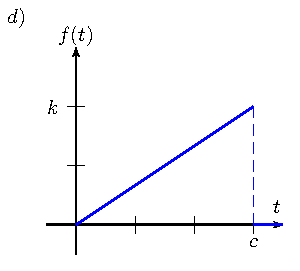
\includegraphics{cap_definicao/pics/figura_7}
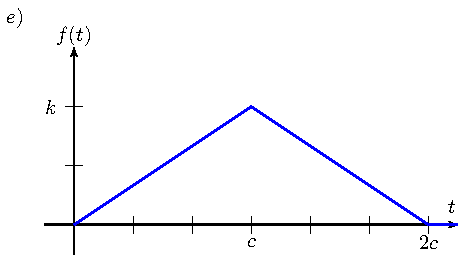
\includegraphics{cap_definicao/pics/figura_8}\end{center}
\end{exer}
\begin{resp}
 \begin{itemize}
  \item[a)] $\displaystyle F(s)=\frac{k}{s}e^{-sc}$
  \item[b)] $\displaystyle F(s)=\frac{k}{s}\left(1-e^{-sc}\right)$ 
  \item[c)] $\displaystyle F(s)=\frac{k}{s}e^{-sc}\left(1-e^{-sb}\right)$ 
  \item[d)] $\displaystyle F(s)=-\frac{k}{c}\left(\frac{c}{s}e^{-sc}+\frac{1}{s^2}\left(e^{-sc}-1\right)\right)$
  \item[e)] $\displaystyle F(s)=\frac{k}{cs^2}\left(1-2e^{-cs}+e^{-2cs}\right)$
 \end{itemize}
\end{resp}
\begin{exer}Use a definição de transformada de Laplace para calcular as transformadas das funções dadas a seguir:
 \begin{itemize}
  \item[a)] $f(t)=at$
  \item[b)] $f(t)=\left\{\begin{array}{ll}0, & 0\leq t< 2\\2,&  2\leq t< 3\\0,&t>3 \end{array}\right.$
  \item[c)] $f(t)=a^t,~~a>0$
  \item[d)] $f(t)=\cos(wt)$ 
  \item[e)] $f(t)=\cosh(at)$ 
  \item[f)] $f(t)=te^{2t}$ 
  \item[g)] $f(t)=e^{-t+4}$ 
 \end{itemize}
\end{exer}
\begin{resp}
 \begin{itemize}
  \item[a)] $F(s)=\frac{a}{s^2}$
  \item[b)] $F(s)=\frac{2}{s}e^{-2s}\left(1-e^{-s}\right)$ 
  \item[c)] $F(s)=\frac{1}{s-\ln(a)}$
  \item[d)] $F(s)=\frac{s}{s^2+w^2}$ 
  \item[e)] $F(s)=\frac{s}{s^2-a^2}$ 
  \item[f)] $F(s)=\frac{1}{(s-2)^2}$ 
  \item[g)] $F(s)=\frac{e^{4}}{s+1}$ 
  \end{itemize}
\end{resp}
 \begin{exer}\label{inducao_tn}(Princípio da Indução) Mostre que $\displaystyle\mathcal{L}\{t^n\}=\frac{n!}{s^{n+1}}$ seguindo os seguintes passos:
 \begin{itemize}
  \item[a)] Mostre que a fórmula é válida para $n=0,\ 1,\ 2$ e $3$.\footnote{De fato, bastaria mostrar para $n=0$.}
  \item[b)] Mostre que $\displaystyle\mathcal{L}\{t^{n-1}\}=\frac{(n-1)!}{s^{n}}$ é válida, então $\displaystyle\mathcal{L}\{t^n\}=\frac{n!}{s^{n+1}}$ também o é.
 \end{itemize}
 \end{exer}

 
\section{Condição de existência da transformada de Laplace}
A integral que define a transformada de Laplace nem sempre converge e, nesse caso, dizemos que a função não possui transformada de Laplace. As funções $f(t)=e^{t^2}$ e $f(t)=\frac{1}{t}$ são alguns exemplo de funções que não possuem transformada de Laplace. Nessa seção, vamos introduzir uma família de funções que possuem transformada de Laplace. Neste contexto, vamos considerar as funções que são contínuas por partes, ou seja, aquelas que possui um número finito de descontinuidade.
\begin{defn}Dizemos que uma função $f(t)$ é de ordem exponencial $c$ se existem constantes $c$, $M>0$ e $T>0$ tal que $|f(t)|\leq M e^{ct}$ para todo $t>T$. 
\end{defn}
\begin{ex}As funções $f(t)=t^2$, $g(t)=\sen(t)$, $h(t)=e^{-t}$ são de ordem exponencial, pois
$$
|t^2|\leq e^t,\qquad t>0,
$$
$$
|5\cos(t)|\leq e^t,\qquad t>2,
$$
$$
|e^{-t}|\leq e^t,\qquad t>0.
$$
A figura \ref{ordem_exp} ilustra o crescimento de $f$, $g$ e $h$
\begin{figure}[!ht]
\begin{center}

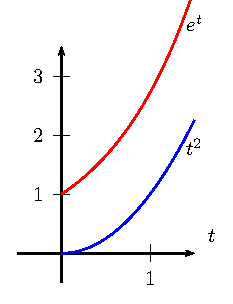
\includegraphics{cap_definicao/pics/figura_1}
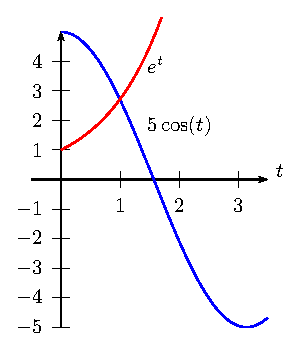
\includegraphics{cap_definicao/pics/figura_2}
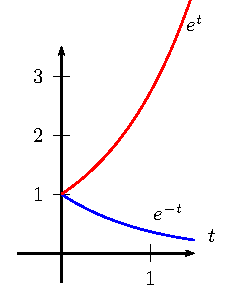
\includegraphics{cap_definicao/pics/figura_3}\end{center}
\caption{\label{ordem_exp}}
\end{figure}
\end{ex}
\begin{teo}\label{ordem_exp_exist} Se $f(t)$ é integrável em cada intervalo $[a,b]\subset[0,\infty)$ e de ordem exponencial $c$, então a transformada de Laplace de $f(t)$ existe para $s>c$.
\end{teo}
\begin{proof}Como a função $f(t)$ é de ordem exponencial $c$, então existem constantes $c$, $M>0$ e $T>0$ tal que $|f(t)|\leq M e^{ct}$ para todo $t>T$. Assim, se $\hat{T}$ é maior ou igual a $T$, a transformada de Laplace  pode ser escrita como a seguinte soma:
$$
\mathcal{L}\{f(t)\}=\int_0^\infty f(t)e^{-st}dt=\int_0^{\hat{T}} f(t)e^{-st}dt+\int_{\hat{T}}^\infty f(t)e^{-st}dt.
$$
A primeira parcela do lado direito é a integral do produto de duas funções integráveis no intervalo $[0, \hat{T}]$, logo, está bem definido. Agora, como $\hat{T}\geq T$, podemos estimar
\begin{eqnarray*}
\left|\int_{\hat{T}}^\infty f(t)e^{-st}dt\right|&\leq& \int_{\hat{T}}^\infty \left|f(t)\right|e^{-st}dt\leq \int_{\hat{T}}^\infty M e^{ct}e^{-st}dt\\
&=&M \int_{\hat{T}}^\infty e^{-(s-c)t}dt
=\left.\frac{M}{c-s} e^{-(s-c)t}\right|_{\hat{T}}^\infty =\frac{M}{s-c}e^{-(s-c)\hat{T}} ,\qquad s>c.
\end{eqnarray*}
Como $\lim_{\hat{T}\to \infty} \frac{M}{s-c}e^{-(s-c)\hat{T}}=0$, a integral $\int_0^\infty f(t)e^{-st}dt$ converge para todo $s>c$, ou seja, a transformada de Laplace existe neste domínio.
\end{proof}
\begin{obs} O teorema \ref{ordem_exp_exist} apresenta condições suficientes para existência da transformada de Laplace, estas condições não são, no entanto, necessárias. Por exemplo, a função $f(t)=\ln(t)$ não é contínua na origem, sequer é limitada quando $t\to 0+$, mas admite uma Transformada de Laplace.
 \end{obs}
\begin{teo} (Comportamento no infinito) Se a transformada de Laplace de uma função limitada $f(t)$ existe, $F(s)=\mathcal{L}\{f(t)\}$, então
$$
\lim_{s\to\infty}F(s)=0.
$$
\end{teo}
\begin{proof}
 Por definição,
 $$
 F(s)=\int_0^\infty f(t)e^{-st}dt.
 $$
Fazendo $u=st$, temos:
$$
 F(s)=\frac{1}{s}\int_0^\infty f\left(\frac{u}{s}\right)e^{-u}du.
 $$
 Usando o fato que $f$ é limitada, existe $M$ tal que $|f(t)|<M$ e, assim,
$$
| F(s) |\leq \frac{M}{s}\int_0^\infty e^{-u}du = \frac{M}{s}.
 $$ 
 Portanto, $|F(s)|\to 0$ quando $s\to \infty$, o que implica 
 $$
\lim_{s\to\infty}F(s)=0.
$$
\end{proof}

\subsection*{Exercícios}
\begin{exer}Identifique quais funções são integráveis por partes e de ordem exponencial, isto é, se enquadram nas hipóteses do teorema \ref{ordem_exp_exist}.
\begin{itemize}
 \item[a)] $f(t)=e^{30t}$.
 \item[b)] $f(t)=e^{-5t}\cos(t) $.
 \item[c)] $f(t)=\frac{1}{t}$.
 \item[d)] $f(t)=\ln(t)$.
 \item[e)] $f(t)=\frac{1}{t^2}$.
  \item[f)] $f(t)=t^{5}+1$.
  \item[g)] $f(t)=e^{-t^2}$.
  \item[h)] $f(t)=e^{t^2}$.

  
  \item[i)] $
f(t)=\left\{\begin{array}{ll} 0, &0\leq t\leq 3\\ 1, & 3\leq t\leq 5,\\0,&t>5.
\end{array}\right.
$
\end{itemize}


\end{exer}


\section{A transformada inversa de Laplace}
Se $F(s)=\mathcal{L}\{ f(t)\}$ é a transformada de Laplace de $f(t)$, então dizemos que $f(t)=\mathcal{L}^{-1}\{ F(s)\}$ é a transformada inversa de Laplace da função $F(s)$. Essa definição só faz sentido se a transformação definida no conjunto de funções que possuem transformada de Laplace for "bijetora", ou seja, cada função $f(t)$ está relacionada a uma única transformada $F(s)$. É fácil observar que duas funções iguais a partir de $t=0$ possuem a mesma transformada de Laplace. Porém, se duas transformadas são iguais para $s>s_0$, por exemplo, $F(s)=G(s)$, então
$$
\int_0^\infty f(t)e^{-st}dt=\int_0^\infty g(t)e^{-st}dt
$$
ou seja,
$$
\int_0^\infty (f(t)-g(t))e^{-st}dt=0
$$
para cada $s>s_0$. Mas, o fato dessa integral ser nula, não significa que a função $f(t)-g(t)$ é nula. Tome como exemplo a função
$$
h(t)=\left\{\begin{array}{ll} 0,& 0\leq t< 3,\\1,& t= 3,\\0,& t> 3,  \end{array}\right.
$$
que não é nula, mas a integral 
\begin{equation}{\label{eq_int_inv}}
\int_0^\infty h(t)e^{-st}dt=0\qquad \forall s>s_0.
\end{equation}
No entanto, a função $f(t)-g(t)$ não pode ser diferente de zero em um conjunto muito grande. Basta tomar como exemplo uma função que não se anula em um intervalo pequeno:
$$
h(t)=\left\{\begin{array}{ll} 1,& 0\leq t< \epsilon,\\0,& t\geq \epsilon  \end{array}\right.
$$
para $0<\epsilon<<1$. Por menor que seja $\epsilon$, a integral (\ref{eq_int_inv}) não se anula para $s>0$. Existe um conceito que diz que duas funções $h_1(t)$ e $h_2(t)$ são iguais quase-sempre em $[a,b]$ se 
$$
\int_a^b |h_1(t)-h_2(t)|dt=0.
$$
Observe que o módulo no conceito é importante, pois podemos tomar uma função diferente de zero em intervalos grandes e com integral zero, por exemplo,
\begin{equation}{\label{eq_lap_inv}}
h_3(t)=\left\{\begin{array}{ll} 1,& 0\leq t< 1,\\-1,& 1\leq t< 2,\\0,& t\geq 2,  \end{array}\right..
\end{equation}
Observe que a integral (\ref{eq_int_inv}) deverá ser zero para todo $s>s_0$, o que compensa a falta do módulo. Por exemplo, a integral (\ref{eq_int_inv}) aplicada a função (\ref{eq_lap_inv}) não é zero:
\begin{eqnarray*}
\int_0^\infty h_3(t)e^{-st}dt&=&\int_0^\epsilon e^{-st}dt-\int_\epsilon^{2\epsilon} e^{-st}dt\\
&=&\left.\frac{ e^{-st}}{-s}\right|_0^\epsilon-\left.\frac{e^{-st}}{-s}\right|_{\epsilon}^{2\epsilon}\\
&=&\frac{1}{s}-\frac{ e^{-s\epsilon}}{s}-\frac{e^{-s\epsilon}}{s}+\frac{e^{-2s\epsilon}}{s}\neq 0,\qquad s>0.
\end{eqnarray*}
Usando esse conceito, se duas transformadas de Laplace são iguais, as respectivas inversas são iguais quase-sempre. Nesse sentido, uma função que possui transformada de Laplace está contida numa classe de funções que possuem a mesma transformada de Laplace. Se olharmos cada classe de funções como um elemento de um conjunto, então a transformada de Laplace é "bijetora". Isso significa que a transformada inversa está bem definida, mesmo que não escrevemos uma forma integral fechada para ela. Uma forma integral fechada para a transformada inversa de Laplace aparecerá naturalmente na teoria de transformada de Fourier.
Abaixo segue a pequena tabela \ref{tab_1} das transformadas de Laplace que calculamos na seção \ref{sec_1} e suas respectivas inversas. Observe que cada função da segunda coluna representa uma classe de funções iguais quase-sempre. As tabelas \ref{tab_trans_Lap_1} e \ref{tab_trans_Lap_2} do apêndice \ref{ap_A} estão mais completas. As tabelas de transformadas são úteis quando estamos resolvendo uma equação diferencial, pois na prática, consultamos uma tabela para calcular a inversa.
\begin{table}
\begin{small}
\begin{center}
\begin{tabular}{|c|c|}
\hline &\\
$\displaystyle F(s)=\mathcal{L }\{f(t)\} $&$\displaystyle  f(t)=\mathcal{L }^{-1}\{F(s)\}$ \\&\\ 
\hline &\\
$\displaystyle \frac{1}{s} $&$\displaystyle  1$ \\ &\\
\hline &\\
$\displaystyle \frac{1}{s^2} $&$\displaystyle  t$ \\ &\\
\hline &\\
$\displaystyle \frac{1}{s^n}, \qquad (n=1,2,3,...) $&$\displaystyle  \frac{t^{n-1}}{(n-1)!}$ \\ &\\
\hline
\end{tabular}
\begin{tabular}{|c|c|}
\hline &\\
$\displaystyle F(s)=\mathcal{L }\{f(t)\} $&$\displaystyle  f(t)=\mathcal{L }^{-1}\{F(s)\}$ \\&\\ 
\hline &\\
$\displaystyle \frac{a}{a^2+s^2} $&$\displaystyle  \sen(at)$ \\ &\\
\hline &\\
$\displaystyle \frac{1}{s+a} $&$\displaystyle  e^{ -at}$ \\ &\\
\hline
\end{tabular}
\caption{\label{tab_1}}
\end{center}
\end{small}
\end{table}
\begin{ex}Para calcular a transformada inversa da função $F(s)=\frac{10}{100+s^2}$, fixamos $a=10$ na quarta linha da tabela \ref{tab_1} e obtemos
$$
\mathcal{L }^{-1}\left\{ \frac{10}{100+s^2}\right\}=\sen(10t)
$$
\end{ex}
\begin{ex}Da mesma forma, para calcular a transformada inversa da função $F(s)=\frac{1}{s^{30}}$, fixamos $n=30$ na terceira linha da tabela \ref{tab_1} e obtemos
$$
\mathcal{L }^{-1}\left\{ \frac{1}{s^{30}}\right\}=\frac{t^{29}}{29!}.
$$
\end{ex}
\subsection*{Exercícios}

 \begin{exer}Use a tabela \ref{tab_trans_Lap_1} para calcular a transformada Inversa de Laplace das funções:
 \begin{itemize}
  \item[a)] $F(s)=\frac{1}{s^2+4}$
  \item[b)] $F(s)=\frac{1}{s^2-4}$
  \item[c)] $F(s)=\frac{s}{s^2-9}$
  \item[d)] $F(s)=-\frac{s}{s^2+2s+1}-\frac{1}{s^2+2s+1}$ 
  \item[e)] $F(s)=\frac{1}{(s^2+2s+1)(s+1)}$ 
 \end{itemize}
\end{exer}
\begin{resp}
 \begin{itemize}
  \item[a)] $f(t)=\frac{1}{2}\sen(2t)$
  \item[b)] $f(t)=\frac{1}{2}\senh(2t)$ 
  \item[c)] $f(t)=\cosh(3t)$
  \item[d)] $f(t)=-e^{-t}$ 
  \item[e)] $f(t)=\frac{t^2e^{-t}}{2}$ 
  \end{itemize}
\end{resp}
